\documentclass{article}
\usepackage[utf8]{inputenc}
\usepackage{graphicx}
\usepackage{multirow}
\usepackage{float}
\usepackage{geometry}
\geometry{
	a4paper,
	total={170mm,257mm},
	left=30mm,
	right=30mm,
	top=20mm,
}
\usepackage{array}
\newcolumntype{L}[1]{>{\raggedright\let\newline\\\arraybackslash\hspace{0pt}}m{#1}}
\newcolumntype{C}[1]{>{\centering\let\newline\\\arraybackslash\hspace{0pt}}m{#1}}
\newcolumntype{R}[1]{>{\raggedleft\let\newline\\\arraybackslash\hspace{0pt}}m{#1}}

\title{Workplan for project A3: Motion Control of Unmanned Aerial Vehicle}

\author{Vilhelm Dinevik \\ Paula Carbó}
\date{\today}

\begin{document}
	\maketitle
	%\newpage
	
	\bigskip
	\tableofcontents
	\newpage
	\section{Background}
		Unmanned aerial vehicles, also known as UAVs, are becoming nowadays more and more popular because they are small, cheap to produce, have low operating and maintenance cost, have great maneuverability, can perform steady flight operations and are able to enter high-risk areas without having to compromise human safety. Most applications that involve UAVs have been used in open areas without any obstacles and with a human in control of the UAV. But in recent years people have come up with more modern applications of UAVs that will need UAVs to fly autonomously in densely populated areas, with a lot of other autonomous UAVs around, e.g. Amazon Prime Air delivery system, AltiGator drones services for inspection and data adquisition, or multi-UAVs used to deploy an aerial communications network. This places high demands on UAVs’ obstacle avoidance capabilities for both moving and static obstacles.
		
		\vspace{1em}
		There are many different manufacturers and a vast amount of different UAV models, all with different motors, weights, sensors and lift-to-weight ratio. To make a standard autonomous flight applicable to all these kinds of UAVs, a simple and easy-to-implement multi-UAV mathematical model, that will still be able to avoid obstacles with as few sensors as possible, is needed.  
		
		\vspace{1em}
		This project aims to study and develop a mathematical model of a quadrotor UAV and the available sensors in it.  From the trajectory and pose tracking a state feedback controller will be designed. In order to facilitate the multi-UAV navigation, potential fields or an A* algorithm will be used to make several quads fly to their goals while maintaining collision avoidance with respect to other quads and obstacles. To check the validity of the models, a simulated test environment in MatLab filled with a random reasonable amount of static obstacles and autonomous UAVs will be used.

	\bigskip
	\section{Goals}	 
	\begin{itemize}
		\item Present a paper/combination of papers that describe the modelling of the UAVs, sensors and tracking. Observe how it is done in the community, categorize these papers and reflect on what our paper contributes with.\\  
		$\rightarrow$ The literature goal can be considered complete when the literature proposed by the supervisor and other interesting documents proposed by the students have been all read, understood and classified, so there are at least 3 papers analysed and compared for each section (modelling of the quad, of the sensors or for the tracking). %not really good enough, don't know what to change it to tho
	
		\item Mathematical Model. Have a robust model for the kinematics and dynamics of the UAV, and its sensors.\\
		$\rightarrow$ The mathematical model goal can be completed when we can describe our UAV with a matrix that includes its position, its linear velocity, its angles (roll, yaw and pitch) and its angular velocity, all of them related to a certain fixed reference frame that we can relate with, for example, the initial frame. Also, when we have derived an equation for each of the necessary sensors: IMU sensor (accelerometer and gyroscope), an 360 degree proximity sensor and GPS. Each model will be tested 3 times on MatLab and the results will be compared to the ones that should be expected.
		
		\item The goal for the control part is to be able to control the trajectory and stability of the UAV. \\
		$\rightarrow$ The control goal can be considered as completed when we are able, for a certain desirable movement of the UAV, to obtain the appropriate force of thrusters for the UAV to achieve the desired position as the UAV stays stable and follows the trajectory vector obtained from the potential fields. The state feedback controller should also satisfy the robustness criteria, observability, controllability and be stable (check poles).
		
		\item When the simulation is completed it should verifie that all the previous steps have been appropriately carried out so the main purpose of the project is achieved. Extract results. \\
		$\rightarrow$ The simulation goal can be tested by testing the proper functioning of the mathematical models that have been implemented with numerical examples. Then we need to test our model, at least in a 2D-simulation and preferably in a 3D-simulation, and we have at least 95\% of our UAVs arriving to their goals without getting stuck and no collisions. 
		
		\vspace{2em}
		%Previously this paragraph was in the project model: work tree section. I think it's more useful to have it here
		 When we have completed the goals for a section in the first level of the work tree we will give a small presentation to our supervisor about that section. We will present the goals we aimed at for that part of the project, the model we came up with or the results we had, and then motivate that we have completed the said goals. This will give us a chance to show that we really understand what we have done and will probably help with the report later on since it'll give us a chance to explain what we have done and why we have come up with those results, just like we will do in the report. The report should be done by the 30th of April, and the rest of the deadlines are specified in the 
	\end{itemize}

	\section{Organization}
	\begin{center}
		\begin{tabular}{|c|c|c|c|} \hline
			%make a table over our organization	
			Member name & E-mail & Telephone number & Position \\ \hline
			Christos Verginis & cverginis@kth.se & 0704438285 & Supervisor \\ \hline
			Vilhelm Dinevik & vdinevik@kth.se & & Student\\ \hline
			Paula Carbó & paulacc@kth.se & +34 626329389 & Student\\ \hline
		\end{tabular}
	\end{center}
	
	
	\section{Project Model}
				\begin{center}
			\begin{tabular}{|C{2cm}|C{2cm}|C{7cm}|C{3cm}|} \hline
				Phase & Sub-phases & Description & Schedule\\ \hline
				Modelling & Quad & Complete the UAV (kinematics and dynamics) mathematical modelling goal. It is done in parallel with the sensors sub-phase. &  1-Feb $\rightarrow$ 4-March  \\ \cline{2-4}
				& Sensors & Complete modelling all the sensors that should be used as to complete the modelling goal. It is done in parallel with the quad sub-phase. & 1-Feb $\rightarrow$ 4-March \\ \hline
				
				Control & Tracking & Make a controller that makes our UAV go in a certain direction with stability. It is the first step of out control phase since it is more related with the previous phase. &  26-Feb $\rightarrow$ 16-Mar\\ \cline{2-4}
				&Navigation & Starts after the tracking so we can work with the potential fields method to obtain the direction the UAV needs to follow, and then check how the tracking is done. When this sub-phasre and the tracking are completed and checked with the simulation, the goal for the control is achieved. & 5-Mar $\rightarrow$ 23-Mar \\ \hline
				
				Multi-agent case & Model & Starts after the single case modelling and control are finished and tested. Work on the model for a multi-UAV scenario. & 26-Mar $\rightarrow$ 6-Apr\\ \cline{2-4}
				&Control & Work on the control for a multi-UAV scenario. The multi-agent case goal is completed after this sub-phase and the model are finished and its effectivity has been checked with a simulation. & 26-Mar $\rightarrow$ 6-Apr \\ \hline
				
				Simulation & & Simulation starts when modelling is finished as to check its validity and complete the modelling goal. Simulation is resumed again when the control has finished to check again its validity and the same for the multi-agent case. Finally, a week is spent to put together all the other parts, and finish all the program and the interface so the simulation goal can be achieved. & 12-Mar $\rightarrow$ 13-Apr \\ \hline
				
				Report & & The report is roughly written during all the other phases, but in the end we will leave 3  weeks specially to focus on finishing the report. It may be modified after the presentation with the feedback, and it should be on time for the final report deadline & 9-Apr $\rightarrow$ 27-Apr \& 8-May $\rightarrow$ 23-May \\ \hline
				
				Presentation & & A whole week is spent when the preliminary report is finished as to make the presentation as best as possible to fit the time we have available. & 30-Apr $\rightarrow$ 4-May \\ \hline
			\end{tabular}
		\end{center}
		\bigskip
		In the case the schedule was not kept, certain phases will overlap another ones, but we will not delay the next phase, so the workload will increase. 
		
		\begin{center}	
			\bigskip
			\begin{tabular}{|C{3cm}|C{3cm}|C{8.5cm}|} \hline
				Milestone & Deadline & Goals \\ \hline
				Status report 1 & 12-Mar & For the first status report, we will have done all the modeling and a half part of the control, which is the main core of the project.\\ \hline
				Status report 2 & 9-Apr & For status report 2, we will be almost done with the final part of the simulation so the project itself will be almost completed. We will focus on organizing and structuring all our work in the report. So the preliminary final report can continue on this second status report. \\ \hline
				Preliminary final report & 30-Apr & It would have been a while since the simulation phase ended and we had time to work exclusively on the report for two weeks, so the report will be correcly structured, al the pases would be explained and the results and conclusions will also be added.\\ \hline
				Presentation & 8-May & We will have a whole week to prepare for the presentation, which means detecting the most important parts that we should include in our slides, the parts that have to be explained the most, what we can skip, and how to organise all this information so it can be easily understood by the audience. The slides also have to be done.\\ \hline
				Final report & 23-May & Improving the report thanks to the feedback obtained with the preliminary report and the presentation.\\ \hline
			\end{tabular}
		
			\vspace{3em}
			\begin{tabular}{|C{6cm}|C{4cm}|} \hline
				Responsibility & Responsible \\ \hline
				Communication with supervisor & Paula Carbó \\ \hline
				Documentation and backups & Vilhelm Dinevik \\ \hline
				Schedule and deadlines & Paula Carbó \\ \hline
				Report writing and follow-up & Vilhelm Dinevik \\ \hline
				Regularly meeting for both students & Paula Carbó \\ \hline
			\end{tabular}
		\end{center}
	
	\section{Risk analysis}
		\begin{tabular}{|L {2.5cm}|C{0.4cm}|C{0.4cm}|C{0.4cm}|R{9.5cm}|} \hline			
			Risks & P & C & R & Counter measure \\ \hline
			Diseases in the group  & 2 & 2 & 4 & Reactive: Rearrange workload \\ & & & & Proactive: Nothing \\ \hline
			Loss of documents and information & 2 & 4 & 8 & Reactive: recollect information again \\ & & & & Proactive: Have bakups for everything, use Google Drive and GitHub \\ \hline
			
			Running out of time & 4 & 2 & 8 & Reactive: Re-evaluate work plan and consult with supervisor \\ & & & & Proactive:  Have a good work plan, check on each other if we'll complete deadlines in time, check more when deadlines are closing in \\ \hline
			
			Bad communication with supervisor & 2 & 2 & 4 & Reactive: Send reminders if we get no answer in x amount of time. \\ & & & & Proactive: Schedule meetings now (once a week for example) and modify these dates if there is no need to meet. Ask supervisor how long 'x amount of time' should be. Plan accordingly\\ \hline
			
			Inappropriate UAV Model & 3 & 3 & 9 & Reactive: Redesign UAV model?
			\\ & & & & Proactive: Test the calculated model with 3 individual tests of simple rotation and movement around and along one axis in a 3D space where the starting and final position is known either on paper or with matlab, check that you get the expected outcome. \\ \hline
			
			Inappropriate sensor Model & & & & Reactive: Check again datasheets for each sensor, obtain the model again, check if other sensors would be more suitable for the UAV application.
			\\ & & & & Proactive: Study exactly what we need to control our drone and obtain the minimum number of sensors that can provide us this data. Choose the best sensors according to their technical specifications so they suit the UAV application the most.\\ \hline
			
			Faulty state feedback controller & 4 & 3 & 12 & Reactive: Redesign the whole controller. damage control!\\ & & & & Proactive: Check the Observability, Controllability, Robustness Criteria and pole placement of the designed State feedback controller.\\ \hline
			
			Potential Field/ A*-algorithm & & & & Reactive: Rewrite the potential fields method, try other algorithms if these two do not work properly.\\
			& & & & Proactive:  \\ \hline %No idea what to write here, how to check if stuff goes haywire
			
			Multi-agent case & & & & Reactive: Rewrite the modelling.\\
			& & & & Proactive: Make sure the mathematical model of the UAV is general enough as to suit different kinds of quads easily.\\ \hline
			
			Simulation & & & &  Reactive: Consider rewriting the modelling, controller and/or the potential fields method\\
			& & & & Proactive: Choose a reasonable linear velocity so it is impossible for two UAVs to collide even if they encounter each other in the opposite direction. Make it easy to extract information and data from the simulation, like the time a flight lasted by the stright distaince between starting point and goal.\\ \hline
			
			Bugs in the matlab code & 4 & 1 & 4 & Reactive: find the section of the bug and implement rubber duck debugging, use each other as the rubber duck. \\
			& & & & Proactive: for every new part that we implement in the code we should retell what that part do and explain it row by row to each other. \\ \hline
			      
		\end{tabular}		
		
		\bigskip
		Every group member is individually responsible for seeing to that the group actually execute proactive countermeasures. Which group member is responsible for what is specified in the organization section. In case a certain risk has no one responsible for it, then it means both students need to make sure they are following the proactive measures and also both will need to apply the reactive measure in case the risk ends up happening.  
 
	\section{Documentation/Communication rules}
	\begin{itemize}
			\item We will use Github and Google drive for documentation. MatLab, Latex and any other code will be stored on GitHub, and the rest will be stored on Google Drive.
			
			\item Meetings with supervisor are scheduled once a week, on Thursday morning. The time and the confirmation for the next week are decided at the end of each meeting. In the case a meeting is cancelled, the designated responsible for communication with supervisor is in charge of scheduling another meeting for the next week or the week after. The purpose of these meetings is ask the supervisor questions or doubts, explain how the project is advancing, present goals accomplished in the case a section of the project plan is finished, check results and ask for how to improve them.
			
			\item Meetings with both students are not fixedly scheduled but regularly scheduled, at least once or twice a week depending on the availability of each one. The purpose of these meetings is advance on the project, distribute work to do for each section in the case the workload could be splitted, check the deadlines for the documents and make sure the work plan is being followed according to the planned schedule, and prepare questions for the supervisor in the case there was any.
			
			\item We checked with our supervisor that in the case we needed something from him, we can send and e-mail, and we are expected to get a response the same day. If we don't get it within a day, we can send a reminder. 
			
			%anything else on this section?
	\end{itemize}

	\appendix
	\section{Appendix}
	
	\subsection{Time line}
		\begin{figure}[H]
			\centering
			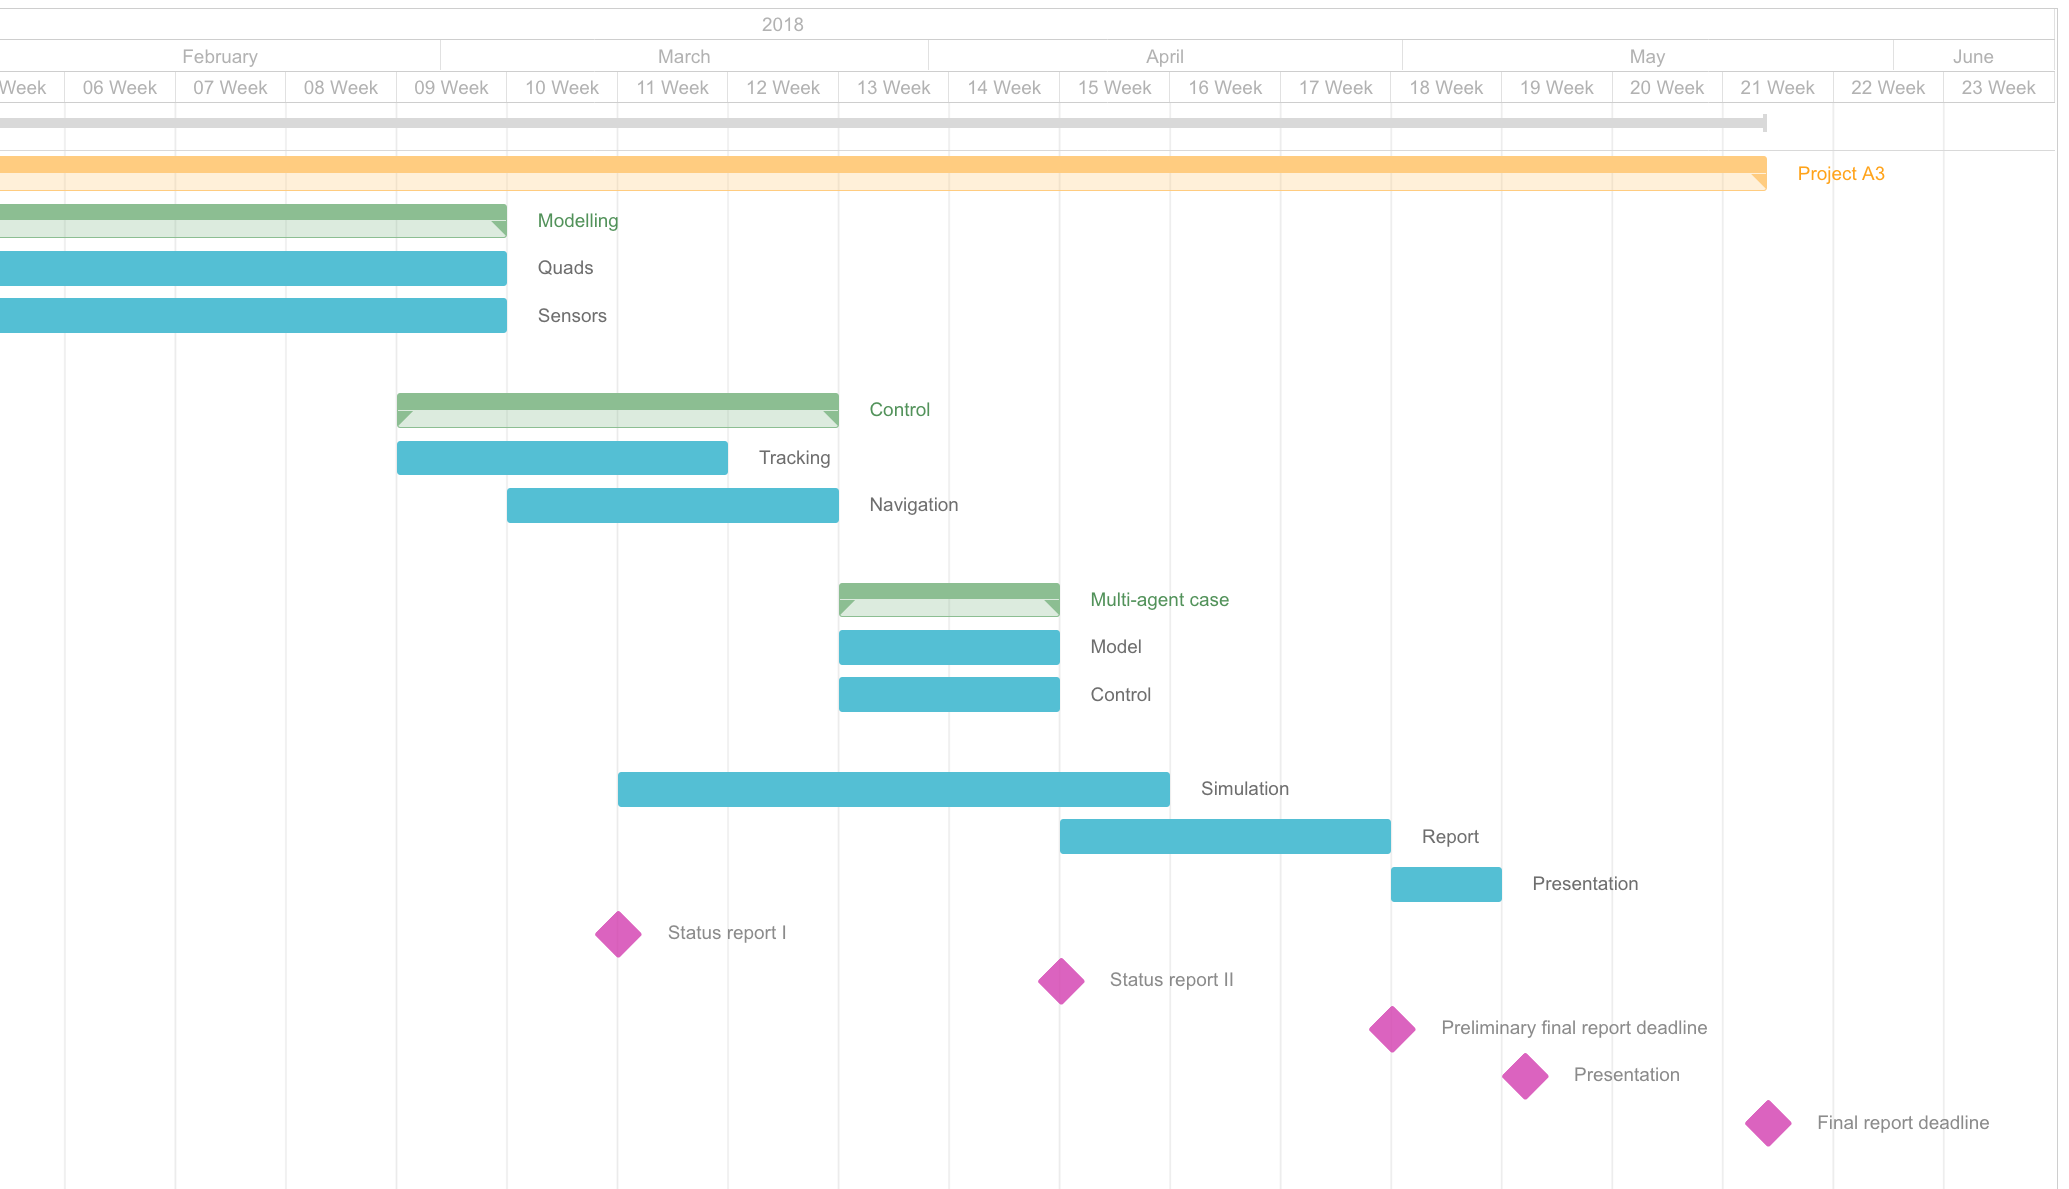
\includegraphics[width=\linewidth]{img/timeline}
			\caption{Time line for the project}
		\end{figure}
		This time line is a visual complement to the table in the project model section. In the mentioned table there is already an explanation on how are the phases related to each other and the milestones.
		
	\subsection{Work tree for the project model}
		\begin{figure}[H]
			\centering
			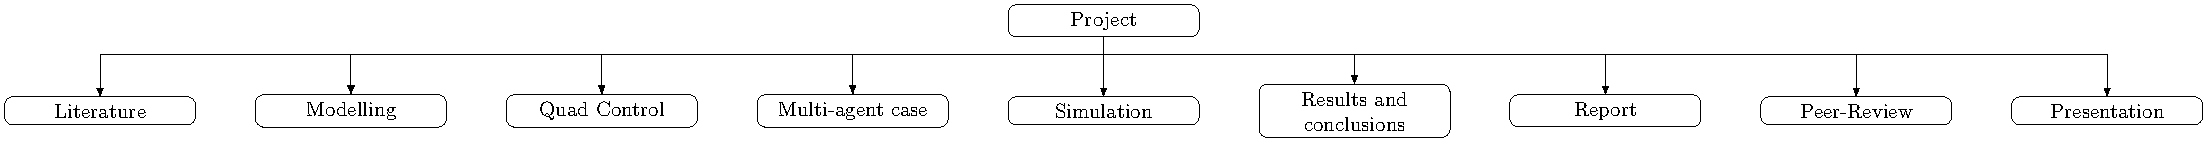
\includegraphics[width=1.15\linewidth]{Workplan_work_tree/basic_work_tree_diagram}
			\caption{First row of work tree}
			\label{fig:work_tree_basic}
		\end{figure}
		\begin{figure}[H]
			\centering
			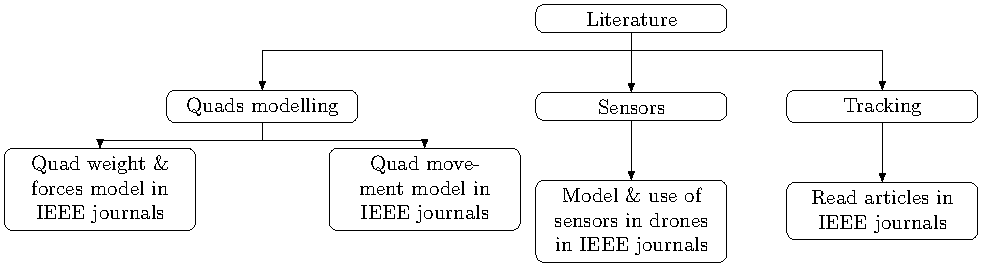
\includegraphics[width=.8\linewidth]{Workplan_work_tree/literature_work_tree_diagram}
			\caption{Expanded work tree for the literature section}
		\end{figure}
		\begin{figure}[H]
			\centering
			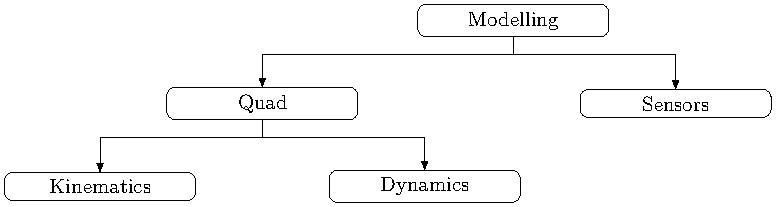
\includegraphics[width=.8\linewidth]{Workplan_work_tree/modelling_work_tree_diagram}
			\caption{Expanded work tree for the modelling section}
		\end{figure}
		\begin{figure}[H]
			\centering
			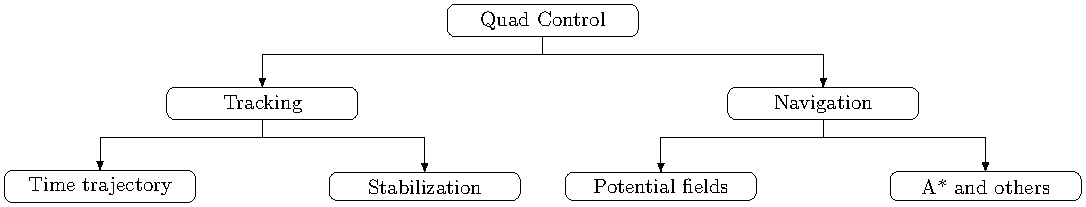
\includegraphics[width=.8\linewidth]{Workplan_work_tree/control_work_tree_diagram}
			\caption{Expanded work tree for the single-quad control section}
		\end{figure}
		\begin{figure}[H]
			\centering
			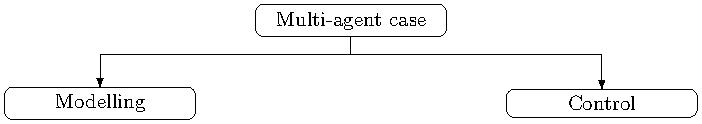
\includegraphics[width=.8\linewidth]{Workplan_work_tree/multiagent_work_tree_diagram}
			\caption{Expanded work tree for the multi-agent case section}
		\end{figure}
		\begin{figure}[H]
			\centering
			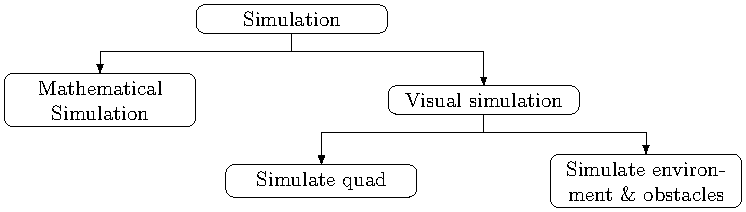
\includegraphics[width=.8\linewidth]{Workplan_work_tree/simulation_work_tree_diagram}
			\caption{Expanded work tree for the simulation section}
		\end{figure}
		
		\paragraph{} We will have a more detailed part of the simulation part of the work tree in status report 1 and a more detailed part of the report and peer-review part in status report 2. 
		
\end{document}
